% https://iitdbgroup.github.io/ProvenanceWeek2021/tapp.html

\documentclass[letterpaper,twocolumn,10pt]{article}
\usepackage{usenix-2020-09}

% to be able to draw some self-contained figs
\usepackage{tikz}
\usepackage{amsmath}

% inlined bib file
% \usepackage{filecontents}
% 
% %-------------------------------------------------------------------------------
% \begin{filecontents}{\jobname.bib}
% %-------------------------------------------------------------------------------
% %
% %
% %
% \end{filecontents}

%-------------------------------------------------------------------------------
\begin{document}
%-------------------------------------------------------------------------------

% don't want date printed
\date{}

% make title bold and 14 pt font (Latex default is non-bold, 16 pt)
\title{\Large \bf A multi-system provenance architecture based on PROV-DM for Explainable AI: Application Track}

% for single author (just remove % characters)
\author{
{\rm Nicholas J. Car}\\
SURROUND Pty Ltd \&\\
Australian National University\\
\href{mailto:nicholas.car@surroundaustralia.com}{nicholas.car@surroundaustralia.com} 
\and
{\rm Robert A. Atkinson}\\
SURROUND Pty Ltd \&\\
Open Geospatial Consortium\\
\href{mailto:rob.atkinson@surroundaustralia.com}{rob.atkinson@surroundaustralia.com} 
} % end author

\maketitle

%-------------------------------------------------------------------------------
\begin{abstract}
%-------------------------------------------------------------------------------
% CFP: https://iitdbgroup.github.io/ProvenanceWeek2021/cfp.html
% Applications Track: need not to focus on novelty but should instead focus on innovative use of provenance and/or deployment of provenance-based solutions and/or open-source software. We invite authors to share insights, experience, and lessons learned when deploying provenance systems. We also encourage submissions describing datasets or tools that could benefit the community.

% Structure: insights, experience, and lessons learned when deploying provenance systems
SURROUND Australia Pty Ltd is a small technology company focused on explainable 
AI and knowledge management products. At the core of our company operations is 
standardised provenance tracking using the PROV Data Model (PROV-DM). Using standardised 
provenance throughout our company lets us both assure customers that any results 
we produce for them are explainable, regardless of the specific systems we employ, 
and also allows us to supply provenance tooling to clients that will work well 
with other logging or provenance systems.

We generate PROV-DM-based provenance in all our important business workflows by 
using either our in-house \textit{ProvWF} tool or workflows within our 
proprietary \textit{SURROUND Ontology Platform} tool. We implement PROV-DM within our 
Knowledge Graph (KG) data products, which are a major part of our business, through the 
\textit{SURROUND Ontology Platform} also and we ''hand off'' provenance tracking 
of some objects to the Git version control system. Our various workflows' and KGs' provenance
information is used together to provide explainable AI results.
\end{abstract}


%-------------------------------------------------------------------------------
\section{Introduction}
%-------------------------------------------------------------------------------
SURROUND Australia Pty Ltd ("SURROUND") is a small technology company founded 6 years ago. While
aiming to supply mainstream AI and knowledge management products to government and private
sector markets, SURROUND attempts to distinguish itself from competitors through sophisticated use
of Semantic Web data due to the belief that such data is the form that best preserves meaning 
over time and system \& organisational change. Specific value propositions for SURROUND's customers, 
based on Semantic Web data use, are:

\begin{itemize}
  \item the expressive power of RDF Schema and OWL2~\cite{dan_brickley_rdf_2014,w3c_owl_working_group_owl_2012} for complex data modelling
  \item the ability to reuse many existing, sophisticated, publishd ontologies directly
  \item the extensibility of RDF graph-based data structures
  \item the systems-independence of Semantic Web data formats
  \item the ability to use a Semantic Web layer to act as a bridge between internal, siloed applications
  \item the ability to share data across organisational boundaries with no inter-organisational special data contracts (due to semantic modelling of all data elements)
  \item the data validation power of modern constraints languages such as SHACL~\cite{knublauch_shapes_2017}
  \item the advanced reasoning capabilities of OWL \& SHACL
\end{itemize}

Emergent from some of these points is SURROUND's ability to provide comensurate provenance information 
across all our different systems due to them all implementing the PROV Data Model (PROV-DM)~\cite{moreau_prov-dm_2013}
in its ontology form, PROV-O~\cite{lebo_prov-o:_2013}, and our ability to produce PROV-O data, to share 
it between applications, to store it and present it.

In this paper we make no new research claim - this is an \textit{Applications Track} paper - but we do aim 
to show ``innovative use of provenance'' and ``the deployment of provenance-based solutions'' that indicate
a certain maturity of approach to the use of provenance for operational tasks. We expect this will be of 
interests to our industry peers and to academics wishing to know where industry implementers are up to
in order to consider next research steps.

We will overview our specific company-wide provenance systems, discuss two projects that use them, indicate 
why we've chosen certain PROV-related implementations over others and where we think some of the provenance
standards need enhancement for our purposes.

%-------------------------------------------------------------------------------
\section{Company-wide provenance architecture}
%-------------------------------------------------------------------------------
SURROUND has a company-wide policy on provenance which is simple that \textit{all} project data processing 
and system operations for clients - work on demand or services supplied - must be recorded in 
PROV-O-compliant forms, with the exception of code and data stored in version control systems which, in all 
instances so far, are implemented in Git\footnote{Git is a free and open source distributed version control 
system, see \url{https://git-scm.com/}}. So far, this policy has been implemented for all our main projects' 
systems and processes, but not for minor projects, some legacy systems or administrative support functions.

Figure~\ref{fig:overview} links types of IT project assets we work with for clients to the tools we implement
to record PROV-O-compliant provenance. 

%-------------------------------------------------------------------------------
\begin{figure*}
  \begin{center}
    \includegraphics[width=\textwidth]{images/overview.png}
  \end{center}
  \caption{\label{fig:overview} SURROUND's provenance tools linked to system type}
  \end{figure*}
%-------------------------------------------------------------------------------

Our major provenance tools, as named in Figure~\ref{fig:overview}, and the actions they perform are:

\begin{itemize}
  \item \textbf{SURROUND Ontology Platform} (SOP)\footnote{\url{https://surroundaustralia.com/sop}}
  \begin{itemize}
    \item an enterprise data management system based on sematic data that is based on Top Quadrant's \textit{EDG}\footnote{\url{https://www.topquadrant.com/products/topbraid-enterprise-data-governance/}}
    \item SOP extends EDG adding the ability to manage various types of semantic assets and collections of them
    \item SOP records PROV-DM provenance for all semantic asset actions
  \end{itemize}
  \item \textbf{ProvWorkflow} (ProvWF)\footnote{\url{https://surroundaustralia.com/provwf}}
  \begin{itemize}
    \item a Python framework and library for the creation of workflows
    \item records PROV-DM provenance for all actions performed by the workflow and all data consumed or produced
    \item supported by SURROUND's \textit{Block Library}
  \end{itemize}
  \item \textbf{Block Library}
  \begin{itemize}
    \item SURROUND's catalogue of ProvWF \textit{Blocks} which are PROV-DM \texttt{Activity} class objects
    \item the library stores many reusable functions within \textit{Blocks}, such as Knowledge Graph API requests, NLP text processing etc.
  \end{itemize}
  \item \textbf{Git}
  \begin{itemize}
    \item we use Git to track the versions of many assets - code, data etc. - in both public and private repositories
    \item although we know of Git-to-PROV mapping tools, e.g. Git2PROV~\cite{tom_de_nies_git2prov_nodate}, we have not yet found it necissary to materialise such mappings but instead record identifiers for versions of PROV-DM \texttt{Entities} using Git and refer to them in PROV-O data
  \end{itemize}\item 
\end{itemize}

In addition to these provenance-specific tools, we implement provenance tracking with general-purpose tools too, such as:

\begin{itemize}
  \item \textbf{RDFlib} (SOP)\footnote{\url{https://github.com/RDFLib/rdflib}}
  \begin{itemize}
    \item a general-purpose RDF manipulation library, written in Python
    \item many of our data objects are RDF graphs
    \item used to create reified provenance for RDF statements     
  \end{itemize}
\end{itemize}  

We ensure provenance information generated by one of our tool is usable in another, for example, \textit{ProfWF}'s outputs
can, and often are, stored in \textit{SOP} which is then able to visualise that provenance either in isolation order
by joining it to other provenance information, perhaps captured by \textit{SOP} itself.


%-------------------------------------------------------------------------------
\section{Footnotes, Verbatim, and Citations}
%-------------------------------------------------------------------------------

Footnotes should be places after punctuation characters, without any
spaces between said characters and footnotes, like so.%
\footnote{Remember that USENIX format stopped using endnotes and is
  now using regular footnotes.} And some embedded literal code may
look as follows.

\begin{verbatim}
int main(int argc, char *argv[]) 
{
    return 0;
}
\end{verbatim}

Now we're going to cite somebody. Watch for the cite tag. Here it
comes. Arpachi-Dusseau and Arpachi-Dusseau co-authored an excellent OS
book, which is also really funny, and
Waldspurger got into the SIGOPS hall-of-fame due to his seminal paper
about resource management in the ESX hypervisor.

The tilde character (\~{}) in the tex source means a non-breaking
space. This way, your reference will always be attached to the word
that preceded it, instead of going to the next line.

And the 'cite' package sorts your citations by their numerical order
of the corresponding references at the end of the paper, ridding you
from the need to notice that, e.g, ``Waldspurger'' appears after
``Arpachi-Dusseau'' when sorting references
alphabetically. 

It'd be nice and thoughtful of you to include a suitable link in each
and every bibtex entry that you use in your submission, to allow
reviewers (and other readers) to easily get to the cited work, as is
done in all entries found in the References section of this document.

Now we're going take a look at Section~\ref{sec:figs}, but not before
observing that refs to sections and citations and such are colored and
clickable in the PDF because of the packages we've included.

%-------------------------------------------------------------------------------
\section{Floating Figures and Lists}
\label{sec:figs}
%-------------------------------------------------------------------------------


%---------------------------
\begin{figure}
\begin{center}
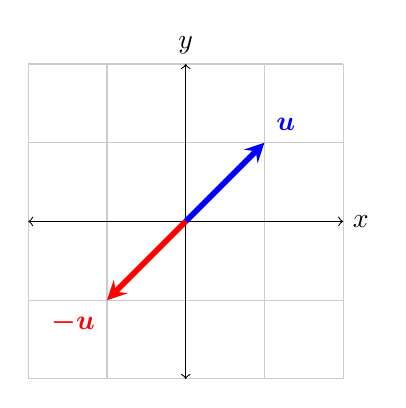
\begin{tikzpicture}
  \draw[thin,gray!40] (-2,-2) grid (2,2);
  \draw[<->] (-2,0)--(2,0) node[right]{$x$};
  \draw[<->] (0,-2)--(0,2) node[above]{$y$};
  \draw[line width=2pt,blue,-stealth](0,0)--(1,1)
        node[anchor=south west]{$\boldsymbol{u}$};
  \draw[line width=2pt,red,-stealth](0,0)--(-1,-1)
        node[anchor=north east]{$\boldsymbol{-u}$};
\end{tikzpicture}
\end{center}
\caption{\label{fig:vectors} Text size inside figure should be as big as
  caption's text. Text size inside figure should be as big as
  caption's text. Text size inside figure should be as big as
  caption's text. Text size inside figure should be as big as
  caption's text. Text size inside figure should be as big as
  caption's text. }
\end{figure}
%% %---------------------------


Here's a typical reference to a floating figure:
Figure~\ref{fig:vectors}. Floats should usually be placed where latex
wants then. Figure\ref{fig:vectors} is centered, and has a caption
that instructs you to make sure that the size of the text within the
figures that you use is as big as (or bigger than) the size of the
text in the caption of the figures. Please do. Really.

In our case, we've explicitly drawn the figure inlined in latex, to
allow this tex file to cleanly compile. But usually, your figures will
reside in some file.pdf, and you'd include them in your document
with, say, \textbackslash{}includegraphics.

Lists are sometimes quite handy. If you want to itemize things, feel
free:

\begin{description}
  
\item[fread] a function that reads from a \texttt{stream} into the
  array \texttt{ptr} at most \texttt{nobj} objects of size
  \texttt{size}, returning returns the number of objects read.

\item[Fred] a person's name, e.g., there once was a dude named Fred
  who separated usenix.sty from this file to allow for easy
  inclusion.
\end{description}

\noindent
The noindent at the start of this paragraph in its tex version makes
it clear that it's a continuation of the preceding paragraph, as
opposed to a new paragraph in its own right.




%-------------------------------------------------------------------------------
\section*{Availability}
%-------------------------------------------------------------------------------

USENIX program committees give extra points to submissions that are
backed by artifacts that are publicly available. If you made your code
or data available, it's worth mentioning this fact in a dedicated
section.

%-------------------------------------------------------------------------------
\bibliographystyle{plain}
% \bibliography{\jobname}
\bibliography{TaPP21}

%%%%%%%%%%%%%%%%%%%%%%%%%%%%%%%%%%%%%%%%%%%%%%%%%%%%%%%%%%%%%%%%%%%%%%%%%%%%%%%%
\end{document}
%%%%%%%%%%%%%%%%%%%%%%%%%%%%%%%%%%%%%%%%%%%%%%%%%%%%%%%%%%%%%%%%%%%%%%%%%%%%%%%%

%%  LocalWords:  endnotes includegraphics fread ptr nobj noindent
%%  LocalWords:  pdflatex acks
